\documentclass[12pt]{article}
\usepackage{fontspec}
\usepackage{fullpage}
\usepackage{hyperref}
\hypersetup{bookmarks=true,colorlinks=true,linkcolor=red,citecolor=blue,filecolor=magenta,urlcolor=cyan}
\usepackage{amsmath}
\usepackage{amssymb}
\usepackage{mathtools}
\usepackage{unicode-math}
\usepackage{tabu}
\usepackage{longtable}
\usepackage{booktabs}
\usepackage{caption}
\usepackage{enumitem}
\usepackage{graphics}
\usepackage{svg}
\usepackage{filecontents}
\usepackage[backend=bibtex]{biblatex}
\usepackage{url}
\setmathfont{Latin Modern Math}
\newcommand{\gt}{\ensuremath >}
\newcommand{\lt}{\ensuremath <}
\global\tabulinesep=1mm
\newlist{symbDescription}{description}{1}
\setlist[symbDescription]{noitemsep, topsep=0pt, parsep=0pt, partopsep=0pt}
\bibliography{bibfile}
\title{Software Requirements Specification for Beam Bending Analysis Program}
\author{Jason Balaci}
\begin{document}
\maketitle
\tableofcontents
\newpage
\section{Reference Material}
\label{Sec:RefMat}
This section records information for easy reference.

\subsection{Table of Units}
\label{Sec:ToU}
The unit system used throughout is SI (Système International d'Unités). In addition to the basic units, several derived units are also used. For each unit, the \hyperref[Table:ToU]{Table of Units} lists the symbol, a description and the SI name.

\begin{longtable}{l l l}
\toprule
\textbf{Symbol} & \textbf{Description} & \textbf{SI Name}
\\
\midrule
\endhead
${\text{m}}$ & length & metre
\\
${\text{N}}$ & force & newton
\\
\bottomrule
\caption{Table of Units}
\label{Table:ToU}
\end{longtable}
\subsection{Table of Symbols}
\label{Sec:ToS}
The symbols used in this document are summarized in the \hyperref[Table:ToS]{Table of Symbols} along with their units. The symbols are listed in alphabetical order.

\begin{longtabu}{l X[l] l}
\toprule
\textbf{Symbol} & \textbf{Description} & \textbf{Units}
\\
\midrule
\endhead
$a$ & A & ${\text{m}}$
\\
${a_{\text{0}}}$ & Coefficient of w\_B's term of power 0 & $\frac{\text{N}}{\text{m}}$
\\
${a_{\text{1}}}$ & Coefficient of w\_B's term of power 1 & $\frac{\text{N}}{\text{m}}$
\\
${a_{\text{2}}}$ & Coefficient of w\_B's term of power 2 & $\frac{\text{N}}{\text{m}}$
\\
${a_{\text{3}}}$ & Coefficient of w\_B's term of power 3 & $\frac{\text{N}}{\text{m}}$
\\
$E$ & Modulus of elasticity of the abstract beam & ${\text{Pa}}$
\\
${E_{B}}$ & Modulus of elasticity of the beam & ${\text{Pa}}$
\\
$f$ & F & ${\text{m}}$
\\
$I$ & Moment of second area of a cross-section of the abstract beam & ${\text{m}}$
\\
${I_{B}}$ & Moment of second area of a cross-section of the beam & ${\text{m}}$
\\
$L$ & Length of the abstract beam & ${\text{m}}$
\\
${L_{B}}$ & Length of the beam & ${\text{m}}$
\\
${w_{B}}$ & Load at a particular point along the beam & ${\text{N}}$
\\
$x$ & One-dimensional point along the beam, from the left-hand side (at the pinned support) & ${\text{m}}$
\\
$y$ & Deflection at a particular point along the abstract beam & ${\text{m}}$
\\
${y_{B}}$ & Deflection at a particular point along the beam & ${\text{m}}$
\\
$ρ$ & Rho & ${\text{m}}$
\\
\bottomrule
\caption{Table of Symbols}
\label{Table:ToS}
\end{longtabu}
\subsection{Abbreviations and Acronyms}
\label{Sec:TAbbAcc}
\begin{longtable}{l l}
\toprule
\textbf{Abbreviation} & \textbf{Full Form}
\\
\midrule
\endhead
BmBnd & Beam Bending Analysis Program
\\
\bottomrule
\caption{Abbreviations and Acronyms}
\label{Table:TAbbAcc}
\end{longtable}
\section{Introduction}
\label{Sec:Intro}


The following section provides an overview of the Software Requirements Specification (SRS) for . This section explains the purpose of this document, the scope of the requirements, the characteristics of the intended reader, and the organization of the document.

\subsection{Purpose of Document}
\label{Sec:DocPurpose}
This document will be used as a starting point for subsequent development phases, including writing the design specification and the software verification and validation plan. The design document will show how the requirements are to be realized, including decisions on the numerical algorithms and programming environment. The verification and validation plan will show the steps that will be used to increase confidence in the software documentation and the implementation. Although the SRS fits in a series of documents that follow the so-called waterfall model, the actual development process is not constrained in any way. Even when the waterfall model is not followed, as Parnas and Clements point out \cite{parnasClements1986}, the most logical way to present the documentation is still to ``fake'' a rational design process.

\subsection{Scope of Requirements}
\label{Sec:ReqsScope}
The scope of the requirements includes .

\subsection{Characteristics of Intended Reader}
\label{Sec:ReaderChars}
Reviewers of this documentation should have an understanding of. The users of BmBnd can have a lower level of expertise, as explained in \hyperref[Sec:UserChars]{Sec:User Characteristics}.

\section{General System Description}
\label{Sec:GenSysDesc}
This section provides general information about the system. It identifies the interfaces between the system and its environment, describes the user characteristics, and lists the system constraints.

\subsection{System Context}
\label{Sec:SysContext}
\subsection{User Characteristics}
\label{Sec:UserChars}
Hello world!.

\subsection{System Constraints}
\label{Sec:SysConstraints}
There are no system constraints.

\section{Specific System Description}
\label{Sec:SpecSystDesc}
This section first presents the problem description, which gives a high-level view of the problem to be solved. This is followed by the solution characteristics specification, which presents the assumptions, theories, and definitions that are used.

\subsection{Problem Description}
\label{Sec:ProbDesc}
A system is needed to .

\subsubsection{Terminology and Definitions}
\label{Sec:TermDefs}
This subsection provides a list of terms that are used in the subsequent sections and their meaning, with the purpose of reducing ambiguity and making it easier to correctly understand the requirements.

\subsubsection{Physical System Description}
\label{Sec:PhysSyst}
The physical system of BmBnd, as shown in \hyperref[Figure:bmbndFull]{Fig:bmbndFull}, includes the following elements:

\begin{figure}
\begin{center}
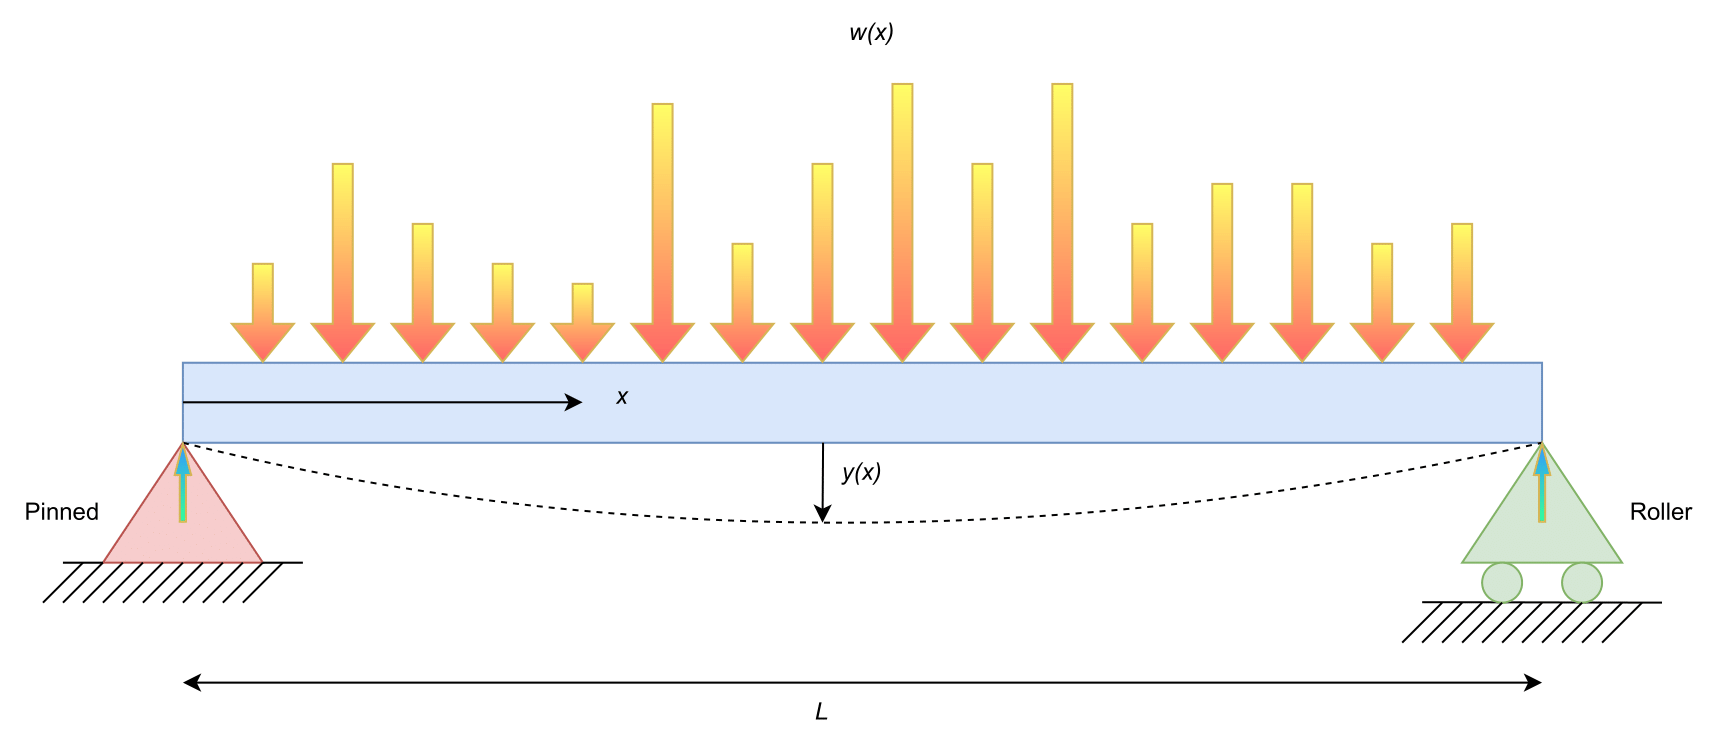
\includegraphics[width=0.7\textwidth]{../../../../datafiles/bmbnd/beam_bending_diagram_annotated.drawio.png}
\caption{physical system}
\label{Figure:bmbndFull}
\end{center}
\end{figure}
\subsubsection{Goal Statements}
\label{Sec:GoalStmt}
Given , the goal statements are:

\begin{itemize}
\item[deflection:\phantomsection\label{deflection}]{Calculate the deflection of the beam under load.}
\end{itemize}
\subsection{Solution Characteristics Specification}
\label{Sec:SolCharSpec}
The instance models that govern BmBnd are presented in the \hyperref[Sec:IMs]{Instance Model Section}. The information to understand the meaning of the instance models and their derivation is also presented, so that the instance models can be verified.

\subsubsection{Assumptions}
\label{Sec:Assumps}
This section simplifies the original problem and helps in developing the theoretical models by filling in the missing information for the physical system. The assumptions refine the scope by providing more detail.

\begin{itemize}
\item[world:\phantomsection\label{world}]{The world model is two-dimensional, observing the instant a load is applied on the beam.}
\item[beamSlender:\phantomsection\label{beamSlender}]{The beam is slender.}
\item[beamPrismatic:\phantomsection\label{beamPrismatic}]{The beam is prismatic.}
\item[beamUniformCrossSection:\phantomsection\label{beamUniformCrossSection}]{The beam has a uniform cross-section.}
\item[beamFlat:\phantomsection\label{beamFlat}]{The beam is flat within a reasonable tolerance.}
\item[beamConstantSecondMomentOfArea:\phantomsection\label{beamConstantSecondMomentOfArea}]{The beam has a constant second moment of area.}
\item[beamVerticalLinearElasticLoad:\phantomsection\label{beamVerticalLinearElasticLoad}]{The beam experiences vertical linear elastic load.}
\item[beamConstantModulusOfElasticity:\phantomsection\label{beamConstantModulusOfElasticity}]{The beam's modulus of elasticity is constant along the beam.}
\item[beamSmallDeflections:\phantomsection\label{beamSmallDeflections}]{Only relatively small deflections will be examined (whereby the maximum deflection is at most SLENDER of the beam's length).}
\item[beamLocallySmallSlopes:\phantomsection\label{beamLocallySmallSlopes}]{The deflection of the beam will have locally small slopes across the beam.}
\item[beamSimplySupported:\phantomsection\label{beamSimplySupported}]{The beam is simply supported.}
\item[beamLoadingPolynomial:\phantomsection\label{beamLoadingPolynomial}]{The beam's loading may be captured by a third-order polynomial of standard form.}
\item[beamNoPointLoads:\phantomsection\label{beamNoPointLoads}]{The beam's loading contains no point loads.}
\item[beamNoAxialLoading:\phantomsection\label{beamNoAxialLoading}]{The beam has no loading applied axially}
\item[beamDeflectionFunctionDifferentiable:\phantomsection\label{beamDeflectionFunctionDifferentiable}]{The beam deflection function is continuously differentiable 4 times on [0, L].}
\item[beamLoadingFunctionIntegrable:\phantomsection\label{beamLoadingFunctionIntegrable}]{The beam loading function is integrable 4 times on [0, L].}
\end{itemize}
\subsubsection{Theoretical Models}
\label{Sec:TMs}
This section focuses on the general equations and laws that BmBnd is based on.

\vspace{\baselineskip}
\noindent
\begin{minipage}{\textwidth}
\begin{tabular}{>{\raggedright}p{0.13\textwidth}>{\raggedright\arraybackslash}p{0.82\textwidth}}
\toprule \textbf{Refname} & \textbf{TM:curvatureThm}
\phantomsection 
\label{TM:curvatureThm}
\\ \midrule \\
Label & Curvature of a plane
        
\\ \midrule \\
Equation & \begin{displaymath}
           \frac{1}{ρ}=\frac{\frac{\,d^{2}f}{\,da^{2}}}{\left(1+\frac{\,df}{\,da}^{2}\right)^{\frac{3}{2}}}
           \end{displaymath}
\\ \midrule \\
Description & \begin{symbDescription}
              \item{$ρ$ is the rho (${\text{m}}$)}
              \item{$a$ is the a (${\text{m}}$)}
              \item{$f$ is the f (${\text{m}}$)}
              \end{symbDescription}
\\ \midrule \\
Source & \hyperref[world]{A:world}
         
\\ \midrule \\
RefBy & 
\\ \bottomrule
\end{tabular}
\end{minipage}
\subsubsection{General Definitions}
\label{Sec:GDs}
There are no general definitions.

\subsubsection{Data Definitions}
\label{Sec:DDs}
This section collects and defines all the data needed to build the instance models.

\vspace{\baselineskip}
\noindent
\begin{minipage}{\textwidth}
\begin{tabular}{>{\raggedright}p{0.13\textwidth}>{\raggedright\arraybackslash}p{0.82\textwidth}}
\toprule \textbf{Refname} & \textbf{DD:loading}
\phantomsection 
\label{DD:loading}
\\ \midrule \\
Label & Load at a particular point along the beam
        
\\ \midrule \\
Symbol & ${w_{B}}$
         
\\ \midrule \\
Units & ${\text{N}}$
        
\\ \midrule \\
Equation & \begin{displaymath}
           {w_{B}}\left(x\right)={a_{\text{0}}}+{a_{\text{1}}} x+{a_{\text{2}}} x^{2}+{a_{\text{3}}} x^{3}
           \end{displaymath}
\\ \midrule \\
Description & \begin{symbDescription}
              \item{${w_{B}}$ is the load at a particular point along the beam (${\text{N}}$)}
              \item{${a_{\text{0}}}$ is the coefficient of w\_B's term of power 0 ($\frac{\text{N}}{\text{m}}$)}
              \item{${a_{\text{1}}}$ is the coefficient of w\_B's term of power 1 ($\frac{\text{N}}{\text{m}}$)}
              \item{$x$ is the one-dimensional point along the beam, from the left-hand side (at the pinned support) (${\text{m}}$)}
              \item{${a_{\text{2}}}$ is the coefficient of w\_B's term of power 2 ($\frac{\text{N}}{\text{m}}$)}
              \item{${a_{\text{3}}}$ is the coefficient of w\_B's term of power 3 ($\frac{\text{N}}{\text{m}}$)}
              \end{symbDescription}
\\ \midrule \\
Source & \hyperref[world]{A:world}
         
\\ \midrule \\
RefBy & 
\\ \bottomrule
\end{tabular}
\end{minipage}

\subsubsection{Instance Models}
\label{Sec:IMs}
This section transforms the problem defined in the \hyperref[Sec:ProbDesc]{problem description} into one which is expressed in mathematical terms. It uses concrete symbols defined in the \hyperref[Sec:DDs]{data definitions} to replace the abstract symbols in the models identified in \hyperref[Sec:TMs]{theoretical models} and \hyperref[Sec:GDs]{general definitions}.

\section{Requirements}
\label{Sec:Requirements}
This section provides the functional requirements, the tasks and behaviours that the software is expected to complete, and the non-functional requirements, the qualities that the software is expected to exhibit.

\subsection{Functional Requirements}
\label{Sec:FRs}
This section provides the functional requirements, the tasks and behaviours that the software is expected to complete.

\begin{itemize}
\item[Input-Values:\phantomsection\label{inputValues}]{Input the values from \hyperref[Table:ReqInputs]{Tab:ReqInputs}.}
\end{itemize}
\begin{longtabu}{l X[l] l}
\toprule
\textbf{Symbol} & \textbf{Description} & \textbf{Units}
\\
\midrule
\endhead
${a_{\text{0}}}$ & Coefficient of w\_B's term of power 0 & $\frac{\text{N}}{\text{m}}$
\\
${a_{\text{1}}}$ & Coefficient of w\_B's term of power 1 & $\frac{\text{N}}{\text{m}}$
\\
${a_{\text{2}}}$ & Coefficient of w\_B's term of power 2 & $\frac{\text{N}}{\text{m}}$
\\
${a_{\text{3}}}$ & Coefficient of w\_B's term of power 3 & $\frac{\text{N}}{\text{m}}$
\\
${E_{B}}$ & Modulus of elasticity of the beam & ${\text{Pa}}$
\\
${I_{B}}$ & Moment of second area of a cross-section of the beam & ${\text{m}}$
\\
${L_{B}}$ & Length of the beam & ${\text{m}}$
\\
\bottomrule
\caption{Required Inputs following \hyperref[inputValues]{FR:Input-Values}}
\label{Table:ReqInputs}
\end{longtabu}
\subsection{Non-Functional Requirements}
\label{Sec:NFRs}
This section provides the non-functional requirements, the qualities that the software is expected to exhibit.

\section{Likely Changes}
\label{Sec:LCs}
This section lists the likely changes to be made to the software.

\section{Traceability Matrices and Graphs}
\label{Sec:TraceMatrices}
The purpose of the traceability matrices is to provide easy references on what has to be additionally modified if a certain component is changed. Every time a component is changed, the items in the column of that component that are marked with an ``X'' should be modified as well. \hyperref[Table:TraceMatAvsA]{Tab:TraceMatAvsA} shows the dependencies of assumptions on the assumptions. \hyperref[Table:TraceMatAvsAll]{Tab:TraceMatAvsAll} shows the dependencies of data definitions, theoretical models, general definitions, instance models, requirements, likely changes, and unlikely changes on the assumptions. \hyperref[Table:TraceMatRefvsRef]{Tab:TraceMatRefvsRef} shows the dependencies of data definitions, theoretical models, general definitions, and instance models with each other. \hyperref[Table:TraceMatAllvsR]{Tab:TraceMatAllvsR} shows the dependencies of goal statements on the data definitions, theoretical models, general definitions, and instance models.

\begin{longtable}{l l l l l l l l l l l l l l l l l}
\toprule
\textbf{} & \textbf{\hyperref[world]{A:world}} & \textbf{\hyperref[beamSlender]{A:beamSlender}} & \textbf{\hyperref[beamPrismatic]{A:beamPrismatic}} & \textbf{\hyperref[beamUniformCrossSection]{A:beamUniformCrossSection}} & \textbf{\hyperref[beamFlat]{A:beamFlat}} & \textbf{\hyperref[beamConstantSecondMomentOfArea]{A:beamConstantSecondMomentOfArea}} & \textbf{\hyperref[beamVerticalLinearElasticLoad]{A:beamVerticalLinearElasticLoad}} & \textbf{\hyperref[beamConstantModulusOfElasticity]{A:beamConstantModulusOfElasticity}} & \textbf{\hyperref[beamSmallDeflections]{A:beamSmallDeflections}} & \textbf{\hyperref[beamLocallySmallSlopes]{A:beamLocallySmallSlopes}} & \textbf{\hyperref[beamSimplySupported]{A:beamSimplySupported}} & \textbf{\hyperref[beamLoadingPolynomial]{A:beamLoadingPolynomial}} & \textbf{\hyperref[beamNoPointLoads]{A:beamNoPointLoads}} & \textbf{\hyperref[beamNoAxialLoading]{A:beamNoAxialLoading}} & \textbf{\hyperref[beamDeflectionFunctionDifferentiable]{A:beamDeflectionFunctionDifferentiable}} & \textbf{\hyperref[beamLoadingFunctionIntegrable]{A:beamLoadingFunctionIntegrable}}
\\
\midrule
\endhead
\hyperref[world]{A:world} &  &  &  &  &  &  &  &  &  &  &  &  &  &  &  & 
\\
\hyperref[beamSlender]{A:beamSlender} &  &  &  &  &  &  &  &  &  &  &  &  &  &  &  & 
\\
\hyperref[beamPrismatic]{A:beamPrismatic} &  &  &  &  &  &  &  &  &  &  &  &  &  &  &  & 
\\
\hyperref[beamUniformCrossSection]{A:beamUniformCrossSection} &  &  &  &  &  &  &  &  &  &  &  &  &  &  &  & 
\\
\hyperref[beamFlat]{A:beamFlat} &  &  &  &  &  &  &  &  &  &  &  &  &  &  &  & 
\\
\hyperref[beamConstantSecondMomentOfArea]{A:beamConstantSecondMomentOfArea} &  &  &  &  &  &  &  &  &  &  &  &  &  &  &  & 
\\
\hyperref[beamVerticalLinearElasticLoad]{A:beamVerticalLinearElasticLoad} &  &  &  &  &  &  &  &  &  &  &  &  &  &  &  & 
\\
\hyperref[beamConstantModulusOfElasticity]{A:beamConstantModulusOfElasticity} &  &  &  &  &  &  &  &  &  &  &  &  &  &  &  & 
\\
\hyperref[beamSmallDeflections]{A:beamSmallDeflections} &  &  &  &  &  &  &  &  &  &  &  &  &  &  &  & 
\\
\hyperref[beamLocallySmallSlopes]{A:beamLocallySmallSlopes} &  &  &  &  &  &  &  &  &  &  &  &  &  &  &  & 
\\
\hyperref[beamSimplySupported]{A:beamSimplySupported} &  &  &  &  &  &  &  &  &  &  &  &  &  &  &  & 
\\
\hyperref[beamLoadingPolynomial]{A:beamLoadingPolynomial} &  &  &  &  &  &  &  &  &  &  &  &  &  &  &  & 
\\
\hyperref[beamNoPointLoads]{A:beamNoPointLoads} &  &  &  &  &  &  &  &  &  &  &  &  &  &  &  & 
\\
\hyperref[beamNoAxialLoading]{A:beamNoAxialLoading} &  &  &  &  &  &  &  &  &  &  &  &  &  &  &  & 
\\
\hyperref[beamDeflectionFunctionDifferentiable]{A:beamDeflectionFunctionDifferentiable} &  &  &  &  &  &  &  &  &  &  &  &  &  &  &  & 
\\
\hyperref[beamLoadingFunctionIntegrable]{A:beamLoadingFunctionIntegrable} &  &  &  &  &  &  &  &  &  &  &  &  &  &  &  & 
\\
\bottomrule
\caption{Traceability Matrix Showing the Connections Between Assumptions and Other Assumptions}
\label{Table:TraceMatAvsA}
\end{longtable}
\begin{longtable}{l l l l l l l l l l l l l l l l l}
\toprule
\textbf{} & \textbf{\hyperref[world]{A:world}} & \textbf{\hyperref[beamSlender]{A:beamSlender}} & \textbf{\hyperref[beamPrismatic]{A:beamPrismatic}} & \textbf{\hyperref[beamUniformCrossSection]{A:beamUniformCrossSection}} & \textbf{\hyperref[beamFlat]{A:beamFlat}} & \textbf{\hyperref[beamConstantSecondMomentOfArea]{A:beamConstantSecondMomentOfArea}} & \textbf{\hyperref[beamVerticalLinearElasticLoad]{A:beamVerticalLinearElasticLoad}} & \textbf{\hyperref[beamConstantModulusOfElasticity]{A:beamConstantModulusOfElasticity}} & \textbf{\hyperref[beamSmallDeflections]{A:beamSmallDeflections}} & \textbf{\hyperref[beamLocallySmallSlopes]{A:beamLocallySmallSlopes}} & \textbf{\hyperref[beamSimplySupported]{A:beamSimplySupported}} & \textbf{\hyperref[beamLoadingPolynomial]{A:beamLoadingPolynomial}} & \textbf{\hyperref[beamNoPointLoads]{A:beamNoPointLoads}} & \textbf{\hyperref[beamNoAxialLoading]{A:beamNoAxialLoading}} & \textbf{\hyperref[beamDeflectionFunctionDifferentiable]{A:beamDeflectionFunctionDifferentiable}} & \textbf{\hyperref[beamLoadingFunctionIntegrable]{A:beamLoadingFunctionIntegrable}}
\\
\midrule
\endhead
\hyperref[DD:loading]{DD:loading} &  &  &  &  &  &  &  &  &  &  &  &  &  &  &  & 
\\
\hyperref[TM:curvatureThm]{TM:curvatureThm} &  &  &  &  &  &  &  &  &  &  &  &  &  &  &  & 
\\
\hyperref[inputValues]{FR:Input-Values} &  &  &  &  &  &  &  &  &  &  &  &  &  &  &  & 
\\
\bottomrule
\caption{Traceability Matrix Showing the Connections Between Assumptions and Other Items}
\label{Table:TraceMatAvsAll}
\end{longtable}
\begin{longtable}{l l l}
\toprule
\textbf{} & \textbf{\hyperref[DD:loading]{DD:loading}} & \textbf{\hyperref[TM:curvatureThm]{TM:curvatureThm}}
\\
\midrule
\endhead
\hyperref[DD:loading]{DD:loading} &  & 
\\
\hyperref[TM:curvatureThm]{TM:curvatureThm} &  & 
\\
\bottomrule
\caption{Traceability Matrix Showing the Connections Between Items and Other Sections}
\label{Table:TraceMatRefvsRef}
\end{longtable}
\begin{longtable}{l l l l}
\toprule
\textbf{} & \textbf{\hyperref[DD:loading]{DD:loading}} & \textbf{\hyperref[TM:curvatureThm]{TM:curvatureThm}} & \textbf{\hyperref[inputValues]{FR:Input-Values}}
\\
\midrule
\endhead
\hyperref[deflection]{GS:deflection} &  &  & 
\\
\hyperref[inputValues]{FR:Input-Values} &  &  & 
\\
\bottomrule
\caption{Traceability Matrix Showing the Connections Between Goal Statements and Other Items}
\label{Table:TraceMatAllvsR}
\end{longtable}
The purpose of the traceability graphs is also to provide easy references on what has to be additionally modified if a certain component is changed. The arrows in the graphs represent dependencies. The component at the tail of an arrow is depended on by the component at the head of that arrow. Therefore, if a component is changed, the components that it points to should also be changed. \hyperref[Figure:TraceGraphAvsA]{Fig:TraceGraphAvsA} shows the dependencies of assumptions on the assumptions. \hyperref[Figure:TraceGraphAvsAll]{Fig:TraceGraphAvsAll} shows the dependencies of data definitions, theoretical models, general definitions, instance models, requirements, likely changes, and unlikely changes on the assumptions. \hyperref[Figure:TraceGraphRefvsRef]{Fig:TraceGraphRefvsRef} shows the dependencies of data definitions, theoretical models, general definitions, and instance models with each other. \hyperref[Figure:TraceGraphAllvsR]{Fig:TraceGraphAllvsR} shows the dependencies of goal statements on the data definitions, theoretical models, general definitions, and instance models. \hyperref[Figure:TraceGraphAllvsAll]{Fig:TraceGraphAllvsAll} shows the dependencies of dependencies of assumptions, models, definitions, requirements, goals, and changes with each other.

\begin{figure}
\begin{center}
\includesvg[width=\textwidth, inkscapelatex = false]{../../../../traceygraphs/bmbnd/avsa}
\caption{TraceGraphAvsA}
\label{Figure:TraceGraphAvsA}
\end{center}
\end{figure}
\begin{figure}
\begin{center}
\includesvg[width=\textwidth, inkscapelatex = false]{../../../../traceygraphs/bmbnd/avsall}
\caption{TraceGraphAvsAll}
\label{Figure:TraceGraphAvsAll}
\end{center}
\end{figure}
\begin{figure}
\begin{center}
\includesvg[width=\textwidth, inkscapelatex = false]{../../../../traceygraphs/bmbnd/refvsref}
\caption{TraceGraphRefvsRef}
\label{Figure:TraceGraphRefvsRef}
\end{center}
\end{figure}
\begin{figure}
\begin{center}
\includesvg[width=\textwidth, inkscapelatex = false]{../../../../traceygraphs/bmbnd/allvsr}
\caption{TraceGraphAllvsR}
\label{Figure:TraceGraphAllvsR}
\end{center}
\end{figure}
\begin{figure}
\begin{center}
\includesvg[width=\textwidth, inkscapelatex = false]{../../../../traceygraphs/bmbnd/allvsall}
\caption{TraceGraphAllvsAll}
\label{Figure:TraceGraphAllvsAll}
\end{center}
\end{figure}
For convenience, the following graphs can be found at the links below:

\begin{itemize}
\item{\hyperref{../../../../traceygraphs/bmbnd/avsa.svg}{}{}{TraceGraphAvsA}}
\item{\hyperref{../../../../traceygraphs/bmbnd/avsall.svg}{}{}{TraceGraphAvsAll}}
\item{\hyperref{../../../../traceygraphs/bmbnd/refvsref.svg}{}{}{TraceGraphRefvsRef}}
\item{\hyperref{../../../../traceygraphs/bmbnd/allvsr.svg}{}{}{TraceGraphAllvsR}}
\item{\hyperref{../../../../traceygraphs/bmbnd/allvsall.svg}{}{}{TraceGraphAllvsAll}}
\end{itemize}
\section{Values of Auxiliary Constants}
\label{Sec:AuxConstants}
There are no auxiliary constants.

\section{References}
\label{Sec:References}
\begin{filecontents*}{bibfile.bib}
@mastersthesis{koothoor2013,
author={Koothoor, Nirmitha},
title={A document drive approach to certifying scientific computing software},
school={McMaster University},
year={2013},
address={Hamilton, ON, Canada}}
@article{parnasClements1986,
author={Parnas, David L. and Clements, P. C.},
title={A rational design process: How and why to fake it},
journal={IEEE Transactions on Software Engineering},
year={1986},
month=feb,
volume={12},
number={2},
pages={251--257},
address={Washington, USA}}
@inproceedings{smithLai2005,
author={Smith, W. Spencer and Lai, Lei},
title={A new requirements template for scientific computing},
booktitle={Proceedings of the First International Workshop on Situational Requirements Engineering Processes - Methods, Techniques and Tools to Support Situation-Specific Requirements Engineering Processes, SREP'05},
year={2005},
editor={Agerfalk, PJ and Kraiem, N. and Ralyte, J.},
address={Paris, France},
pages={107--121},
note={In conjunction with 13th IEEE International Requirements Engineering Conference,}}
\end{filecontents*}
\nocite{*}
\bibstyle{ieeetr}
\printbibliography[heading=none]
\end{document}
